% ==========================================
% AutoExtraction Source: 02-16-monday.mp4
% Model: gemini-3-flash-preview
%
% MERGED AND CLEANED by Gemini Code Assist on 2026-05-01
% This file combines TEIL 1 and TEIL 2 to create a coherent transcript,
% removing redundant overlapping sections and TEIL 3.
% ==========================================

\chapter{Monday: February 16th 2026 \& Real Analysis }


\begin{nice-box}[Context]
This lecture marks the beginning of \emph{Analysis II: mehrere Variablen} (Multivariable Calculus) for the Spring 2026 semester at ETH Zürich. The lecturer, Joaquim Serra, introduces the course structure, logistics, and provides a high-level overview comparing the fundamental goals of Analysis I (single-variable calculus) with the upcoming objectives of Analysis II (vector calculus and higher-dimensional integration).
\end{nice-box}

% ==========================================
% SECTION 1: INTRODUCTION AND LOGISTICS
% ==========================================
\section{Introduction and Administrative Information}

\begin{spoken-clean}[00:00:00 - 00:01:20]
Good morning. Good morning. Thank you. Please, please, please. Uh, good morning and welcome to Analysis 2. Uh, I have here a projection with my name, Joaquim Serra, the name of the coordinator, Enric Florit-Simón. Now, this is my introduction. Um, and then you know the times of the lectures, obviously, because you are here. Um, and I wanted to share before starting with the mathematical content some practical informations that are very important because we are a large group and the — the communication and everything needs to be done in a more or less structured way. Otherwise, otherwise we collapse.
\end{spoken-clean}

\begin{meta-note}[Projected Content]
The lecturer displays the course website for \qt{Analysis II: mehrere Variablen Spring 2026}. Key details shown:
\begin{description}
    \item[Lecturer:] Joaquim Serra
    \item[Coordinator:] Enric Florit-Simón
    \item[Lectures:] Mon 08:15--10:00 (ETA F 5), Wed 08:15--10:00 (HG F 7 / HG F 5), Thu 16:15--18:00 (ETA F 5).
\end{description}
\end{meta-note}

\begin{spoken-clean}[00:01:20 - 00:03:30]
So, as I guess you did — so as a general rule, uh, everything that applied to Analysis 1 applies to Analysis 2, unless otherwise stated. We will try to follow the same rules and then you know what to expect. In particular, you will have this, um, metadata page that I can see that from — from up there is a bit difficult to see, right? But I will try to put it bigger, yeah. Um, so you know that you need to register for the exercise classes. Uh, for the communication, please try to use whenever possible the forum. We will look at the forum and — and reply, and also your — your peers can also reply to questions because many — so then we can use the collective knowledge, right? Um, there will be recordings of the lecture, but not until the later on, okay? Because, uh, is important for the lecture and for you, but mainly, I mean, for you is your interest, uh, if you want to come or not. But for the lecture is very good that you come to the lecture, you ask questions, you stop me when I'm going too fast, these kind of things. You know, it's very important. So it's a — and also is where you meet with your peers and you can communicate, ask questions to your peers. It's — it's — it's better for the learning.
\end{spoken-clean}

\begin{spoken-clean}[00:03:30 - 00:05:07]
Um, we will tell you more about the exam later on, right? Today I will tell you a bit more what is important to be successful in the course, what to expect about this course, and, uh, the details and the rules of the exam will come later on. You don't need to know now. The bonus, there is a $0.25$ bonus, will be in questions that you will answer in some exercise classes. We will tell you in advance which ones. And, uh, essentially you need to be in the — in the exercise class and answer it. And, uh, do not worry because, uh, the — the rule will be thought — in any case it's just $0.25$ points — uh, but the rules will be thought so that if you miss one day or casuistics like this, it's not that you get zero points, right? Okay. Um, lecture notes. There will be lecture notes similar to those in Analysis 1, and we will put them in this page, hopefully by the end of each week, because I — I update them after the lecture, mainly depending on your questions, depending on your feedback. And that's it, uh, I think that the rules are mainly those and the — the organization. Is there some question, uh, about organization? So essentially, as I said, uh, if you have doubts, uh, is like in Analysis 1, unless I say something that is surprising to you, as in Analysis 1. Is it okay, this? Yeah. Okay, now I will switch — I have some other things I want to project later, but now, because we cannot record at the same time blackboard and projection, I will switch one moment to the blackboard. \inlinemetanote{The lecturer turns off the projector and prepares the blackboard} So I can mute, I think. Yeah. Okay. Now we need the light. \inlinemetanote{Adjusts classroom lighting} Okay. Ah, I think that there is already on. Okay.
\end{spoken-clean}

% ==========================================
% SECTION 2: OVERVIEW - ANALYSIS I VS II
% ==========================================
\section{Overview: Analysis I vs. Analysis II}

\begin{spoken-clean}[00:05:07 - 00:07:20]
Okay, now, just to start, um, we will give a very quick, so quick that is almost a cartoon, but a very quick overview of what is Analysis 1 and Analysis 2, right? It's very, very quick. \inlinemetanote{Starts writing on the left blackboard} So, Analysis 1. Um, is — sorry, but for me is very difficult to write big and then it's — so — so if — if you don't see something, I will try to say at loud everything I write, but if — if something — I mean, Analysis is... so, um, Analysis 1, calculus, sorry, it's the first day, right? Bear with me. Calculus is written — is spelled correctly? Yeah. Calculus of one variable, right? And then, if I ne — if — if we had to choose a representative theorem of Analysis 1 that a bit represents the course, uh, what would you choose? So, can you tell me — I know it's the first day, but let's start a bit of communication. Can you tell me at least two answers — so two people can tell me what is the representative — one representative theorem of Analysis 1? Yeah?
\end{spoken-clean}

\begin{student-question}
Fundamental Theorem of Calculus.
\end{student-question}

\begin{spoken-clean}[continued]
Yeah. I agree. Some other representative theorem? He said the Fundamental Theorem of Calculus. Makes sense, right? Okay, after — is there some other guess? Is — yeah, there?
\end{spoken-clean}

\begin{student-question}
The Intermediate Value Theorem.
\end{student-question}

\begin{spoken-clean}[continued]
The Intermediate Value Theorem. Okay. I think we need to use this for the recording, otherwise I — I will repeat. \inlinemetanote{Referring to the catch-box microphone} Later on when I get — I get better with the throwing the — we will use that. So, okay, so fundamental — so we said two theorems that are — that are indeed important. Perhaps the most representative, I would agree and — and I saw many people saying yes, so is the Fundamental Theorem of Calculus, right? And is this... \inlinemetanote{Starts writing the formula on the board}
\end{spoken-clean}

\begin{nice-box}[Board Action: The Fundamental Theorem of Calculus]
The lecturer writes the Fundamental Theorem of Calculus (FTC) on the board. He initially makes a common sign error in the subtraction, which is subsequently corrected.
\end{nice-box}

\begin{math-stroke}[The Fundamental Theorem of Calculus (Recall)]
\begin{ai-type-check-invisible-content}
% f: [a, b] \to \mathbb{R} is differentiable.
% f' is Riemann integrable.
\end{ai-type-check-invisible-content}
In Analysis I, the central result is the Fundamental Theorem of Calculus (FTC), which relates the integral of a derivative to the values of the function at the boundaries:
\[ \text{FTC} \qquad \int_{a}^{b} f'(x) \, dx = \textcolor{red}{f(a) - f(b)} \quad \text{\textcolor{red}{(Incorrect)}} \]
\end{math-stroke}

\begin{spoken-clean}[00:08:35 - 00:08:50]
Is it correct? Yeah, looks like... \inlinemetanote{Pauses and looks at the board} Yeah, there is some mistake? \inlinemetanote{Corrects the board} Good, well spotted.
\end{spoken-clean}

\begin{math-stroke}[The Fundamental Theorem of Calculus (Corrected)]
The corrected statement of the theorem:
\[ \text{FTC} \qquad \int_{a}^{b} f'(x) \, dx = f(b) - f(a) \]
\end{math-stroke}

\begin{spoken-clean}[00:08:50 - 00:10:32]
Now, to — to unfold and to write and to understand every detail about this equation over here, you needed to introduce a lot of things. You needed to define what is that (i.e., the derivative $f'$), right? What is this (i.e., the Riemann integral $\int_{a}^{b}$)? And even — and you spent a lot of time, right? — what is that (i.e., the real numbers $\mathbb{R}$)? It was not — it was not easy. Yeah. Okay, so this is a fairly, fairly compact theorem, yet the ingredients you had to learn, uh, to unfold all of this and to understand the meaning of every symbol here were a bit of work. Now, how will Analysis 2 look like? \inlinemetanote{Moves to   the next section of the board} So this will be calculus, calculus, still calculus in, uh, more than one variable. Well, since you already know one, let's say at least two variables, because otherwise is already covered by Analysis 1. And some representative theorem that would be the equivalent — so the counterpart of this one (i.e., the FTC) — is the Gauss — it has many names, and is always the same theorem. So but — so is the Gauss, Stokes, uh, what else? Divergence, sometimes is called the Divergence Theorem. Uh, and — and that's it, I think. Green, sometimes Green Theorem.
\end{spoken-clean}

\begin{math-stroke}[Analysis II: The Goal]
Analysis II extends these concepts to higher dimensions:
\begin{description}
    \item[Analysis 1:] Calculus of one variable.
    \item[Analysis 2:] Calculus in $\ge 2$ variables.
\end{description}
The representative results in Analysis II are a family of related theorems:
\begin{itemize}
    \item Gauss Theorem
    \item Stokes Theorem
    \item Divergence Theorem
    \item Green Theorem
\end{itemize}
\end{math-stroke}

\begin{spoken-clean}[00:10:32 - 00:11:00]
And now I will write the theorem, and you will not understand exactly what each thing means. I will tell you intuitively, and then the goal of the lecture will be at the end of the lecture you will be able to understand in full precision everything that I wrote here. Okay? So the theorem goes as follows. So we have — we have the space, the space, let's say I will put it in the space $\mathbb{R}^3$. Three coordinates of space, right? This thing... \inlinemetanote{Draws a 3D coordinate system on the board}
\end{spoken-clean}

\begin{math-stroke}[Visualizing the Higher-Dimensional Space]
\begin{center}
\begin{tikzpicture}[scale=1.2, node distance=0.5cm]
% \begin{ai-tikz-planner-invisible-content}
% 1. Background: 3D Axes (x, y, z).
% 2. Midground: A generic 3D volume Omega (the "potato").
% 3. Foreground: Labels for the axes and the volume.
% \end{ai-tikz-planner-invisible-content}
    % 3D Axes
    \draw[->, thick] (0,0,0) -- (2,0,0) node[right] {$x$ (or $x_1$)};
    \draw[->, thick] (0,0,0) -- (0,2,0) node[above] {$z$ (or $x_3$)};
    \draw[->, thick] (0,0,0) -- (0,0,2) node[below left] {$y$ (or $x_2$)};
    
    \node[below right] at (2.5, 2.5, 0) {$\mathbb{R}^3$};
\end{tikzpicture}
\end{center}
\end{math-stroke}

% [SYSTEM] Segment complete. Please prompt "Continue" for the remainder of the segment.
\begin{spoken-clean}[00:11:00 - 00:12:28]
Right? And then in the — in this space (i.e., $\mathbb{R}^3$) we are given a domain, we are given some — or some surface that encloses some interior — so this — this is the interior of the surface and the exterior. Exterior. And this is a surface, right? The surface I call it $S$. What is a surface? It could be a sphere, it could be a sort of — the skin of a \qt{potato}. It's a surface. Two-dimensional object. Right? It has and — and what I'm — this kind of surface will have a interior and a exterior. And the interior of the surface — so the — if the surface is the skin of the potato, the filling of the potato, the white part, right? Is $\Omega$. I call it $\Omega$.
\end{spoken-clean}

\begin{math-stroke}[Visualizing the Domain and Surface]
\begin{ai-tikz-planner-invisible-content}
% 1. Background: 3D Axes (x, y, z).
% 2. Midground: The 3D "potato" volume Omega, drawn with a semi-transparent fill.
% 3. Foreground: The surface S (boundary of Omega) and labels.
\end{ai-tikz-planner-invisible-content}
\begin{center}
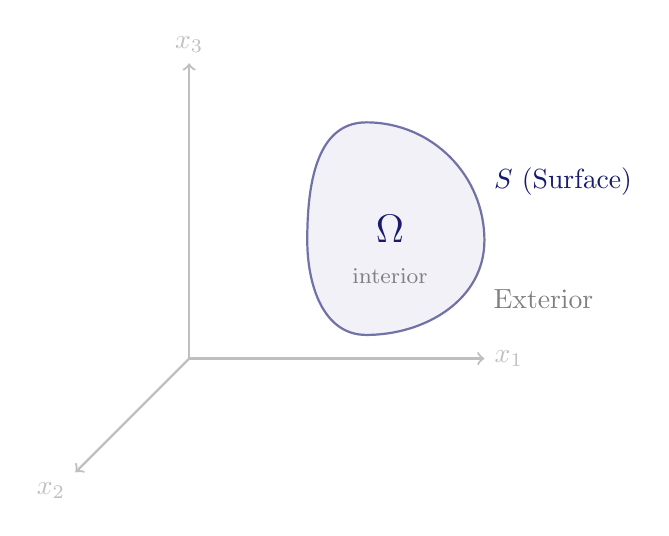
\begin{tikzpicture}[scale=1.5, node distance=0.5cm]
    % 3D Axes
    \draw[->, thick, gray!50] (0,0,0) -- (2.5,0,0) node[right] {$x_1$};
    \draw[->, thick, gray!50] (0,0,0) -- (0,2.5,0) node[above] {$x_3$};
    \draw[->, thick, gray!50] (0,0,0) -- (0,0,2.5) node[below left] {$x_2$};

    % The Potato (Omega)
    \draw[thick, MidnightBlue, fill=MidnightBlue!10, opacity=0.6] 
        (1,1,0) to[out=90,in=180] (1.5,2,0) 
        to[out=0,in=90] (2.5,1,0) 
        to[out=-90,in=0] (1.5,0.2,0) 
        to[out=180,in=-90] cycle;
    
    % Labels
    \node[MidnightBlue] at (1.7, 1.1, 0) {\Large $\Omega$};
    \node[MidnightBlue, right] at (2.5, 1.5, 0) {$S$ (Surface)};
    \node[gray] at (3, 0.5, 0) {Exterior};
    \node[gray] at (1.7, 0.7, 0) {\footnotesize interior};
\end{tikzpicture}
\end{center}
\begin{explanation-of-steps}
The lecturer uses the \qt{potato} analogy to describe a bounded volume $\Omega \subset \mathbb{R}^3$ enclosed by a two-dimensional surface $S = \partial \Omega$. This geometric setup is foundational for the higher-dimensional versions of the Fundamental Theorem of Calculus.
\end{explanation-of-steps}
\end{math-stroke}

\begin{spoken-clean}[00:12:28 - 00:13:32]
And then the equivalent of this theorem (i.e., the FTC) in this setup is this. Given a vector field — now you don't know what it is a vector field, let me tell you. $f$ equal $f_1, f_2, f_3$. These are three — three functions of the space, right? At each point of space you have three numbers. Here you have three numbers, here you have three numbers. Yeah. This is a vector field and how we — do we draw vector fields? Um, we draw it like this, right? It's like a — a field of some cereal, right? But the — in every point you have an arrow instead of a — a plant.
\end{spoken-clean}

\begin{math-stroke}[Defining the Vector Field]
A vector field $f$ assigns a vector to every point in space:
\[ f = (f_1, f_2, f_3) \]
where each $f_i: \mathbb{R}^3 \to \mathbb{R}$ is a scalar function.

\begin{center}
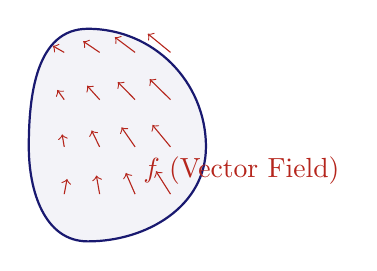
\begin{tikzpicture}[scale=1.5]
% \begin{ai-tikz-planner-invisible-content}
% 1. Background: The potato volume Omega.
% 2. Foreground: A non-uniform vector field F drawn inside the volume.
% \end{ai-tikz-planner-invisible-content}
    % The Potato (Omega)
    \draw[thick, MidnightBlue, fill=MidnightBlue!5] 
        (1,1) to[out=90,in=180] (1.5,2) 
        to[out=0,in=90] (2.5,1) 
        to[out=-90,in=0] (1.5,0.2) 
        to[out=180,in=-90] cycle;
    
    % Vector Field F (Arrows inside)
    \foreach \x in {1.3, 1.6, 1.9, 2.2}
        \foreach \y in {0.6, 1.0, 1.4, 1.8}
            {
                \pgfmathsetmacro{\u}{0.2*cos(\x*50 + \y*30)}
                \pgfmathsetmacro{\v}{0.2*sin(\x*40 - \y*20)}
                \draw[->, BrickRed, thin] (\x,\y) -- (\x+\u, \y+\v);
            }
    
    \node[BrickRed] at (2.8, 0.8) {$f$ (Vector Field)};
\end{tikzpicture}
\end{center}
\end{math-stroke}

\begin{spoken-clean}[00:13:32 - 00:15:15]
Okay, so this is the vector field $f$. And the theorem says that the integral in $\Omega$ of the — the derivative of the field, the $i$ component with respect to the $x_i$ variable, and you sum over $i$. This is equal to the flux of the field across the boundary, across the $S$. And it's called like this. Is $f \cdot \nu$ differential of surface. This is the same theorem you have got here in one dimension (Recall: FTC) in several variables.
\end{spoken-clean}

\begin{math-stroke}[The Divergence Theorem (Gauss's Theorem)]
The \qt{final boss} of Analysis II relates the volume integral of the divergence to the surface integral of the flux:
\begin{color-box}{Black}[Divergence Theorem]
\[ \int_{\Omega} \left( \sum_{i} \frac{\partial f_i}{\partial x_i} \right) \, dx = \int_{S} f \cdot \nu \, dS \]
\end{color-box}

\begin{explanation-of-steps}
This equation is the higher-dimensional analogue of the Fundamental Theorem of Calculus. It states that the total \qt{source} or \qt{sink} of a vector field within a volume $\Omega$ (the left side) is exactly equal to the net flow or \qt{flux} of that field through the enclosing surface $S$ (the right side).
\end{explanation-of-steps}
\end{math-stroke}

\begin{spoken-clean}[00:15:15 - 00:17:38]
Now the small problem is that maybe some of you in physics or — or in previous courses have seen some of these notations, probably not. I don't expect you to — we — and we will need to introduce each of these notations. These partial derivatives, what is a domain, what is a surface? What is this surface mathematically? How do you model a surface? How do you compute a integral over a surface? You know how to compute a integral over the real line, right? Over a segment, but over a surface? This will need some definition and some work. And these objects that are the partial derivatives. So here in — in one equation you have a bit the goal and the syllabus of the course. How will — how will we proceed? So first, we will start looking at the space. In Analysis 1, you did everything in $\mathbb{R}$. Now we will need to introduce $\mathbb{R}^3$, but we are mathematicians so we will — well, some of us. Some of you are physicists or are proto-physicists, would like to become physicists. So we will use this because we don't want to spend time proving the same theorem in — in the plane $\mathbb{R}^2$, then in $\mathbb{R}^3$ in the space, and then when you go to do general relativity you need $\mathbb{R}^4$, right? We do everything in $\mathbb{R}^n$. $n$ is the dimension. So what is $\mathbb{R}^n$? Is the set of $n$ — $n$-tuples of real numbers. This is a definition. Okay? And what is — this is the same as the set of points — we will denote a point $x$, but now $x$ will carry $n$ coordinates. $x_1, x_2, \dots, x_n$. Now this is a point. And these $x_i$ are real numbers. This you know probably because you — you are doing or you have done linear algebra, right? So this should be quite familiar. But still is good that we recall.
\end{spoken-clean}

\begin{math-stroke}[Definition of \texorpdfstring{$\mathbb{R}^n$}{Rn}]
\begin{definition}[The Space $\mathbb{R}^n$]
The space $\mathbb{R}^n$ is defined as the set of all $n$-tuples of real numbers:
\[ \mathbb{R}^n = \{ n\text{-tuples of real numbers} \} \]
Formally, a point $x \in \mathbb{R}^n$ is represented by its coordinates:
\[ x = (x_1, x_2, \dots, x_n) \quad \text{where } x_i \in \mathbb{R} \text{ for all } i \in \{1, \dots, n\} \]
\end{definition}
\end{math-stroke}

\begin{spoken-clean}[00:17:38 - 00:21:13]
Okay. Now, the first part of the course we will be studying $\mathbb{R}^n$ and the properties of $\mathbb{R}^n$. The same a bit as in $\mathbb{R}$ you studied the — the axiom of the supremum, right? Or the — the fact that you can take, uh, limits of Cauchy sequences, these kind of facts, right? The same we will need to study in $\mathbb{R}^n$. Then there will be some new things or — or things that you could also study in $\mathbb{R}$ but become very trivial and now will be much more interesting is the topology of $\mathbb{R}^n$. So first, the $\mathbb{R}^n$ as a space, as Euclidean space. So this is a bit the syllabus. 2: the topology of $\mathbb{R}^n$. You will see what this means indeed, the topology. Then 3: this object over here \inlinemetanote{points at the partial derivatives in the Divergence Theorem} (i.e., the partial derivatives). Partial derivatives. So when you have — when you have several variables you can differentiate a quantity with respect to each of them, right? And differential and — so the differentiation of functions of several variables. Then 4: integration. Integration in $\mathbb{R}^n$, here in a domain of $\mathbb{R}^n$, and on surfaces. But because we want to learn also how to integrate on surfaces, we will do a bit of introduction to differential geometry. Introduction to, uh, surfaces and \qt{submanifolds}. Now I know it's a lot of words, but we will introduce one by one. So surface is a usual two-dimensional object, right? Typically smooth. When it is a three-dimensional object in $\mathbb{R}^4$, for instance, we call this a submanifold. You can also call it surface but — but it's more precise the word submanifold. Or — or — or some two-dimensional object in a five-dimensional space. The — any — any combination of dimensions. And then when you know this, when you know, uh, yes, you will need to know how to integrate. Integration over $\mathbb{R}^n$ and surfaces.
\end{spoken-clean}

\begin{math-stroke}[Course Syllabus]
The roadmap for Analysis II consists of five major pillars:
\begin{enumerate}
    \setcounter{enumi}{0} \item $\mathbb{R}^n$ as Euclidean space.
    \setcounter{enumi}{1} \item Topology of $\mathbb{R}^n$.
    \setcounter{enumi}{2} \item Partial derivatives and differentiation of multivariable functions.
    \setcounter{enumi}{3} \item Introduction to surfaces and \qt{submanifolds} (Differential Geometry).
    \setcounter{enumi}{4} \item Integration over $\mathbb{R}^n$ and surfaces.
\end{enumerate}
\end{math-stroke}

\begin{spoken-clean}[00:21:13 - 00:22:00]
And hopefully then you will know all of these elements. This element, uh, this is the normal vector. This I can tell you now what is this. This is just the vector, the unit vector, the vector of length one that is normal to the surface, right? If you have a surface, this — this $\nu$ is just the — the normal to the surface. So this is easy. Um, but still we will — we will define this in detail. And after we know all of these, we will be able to prove that equation over here (i.e., the Divergence Theorem) and work with it and see why it is useful. Right? For many things. Okay. Uh, so this is a rough plan of the course.
\end{spoken-clean}

\begin{math-stroke}[The Normal Vector]
\begin{center}
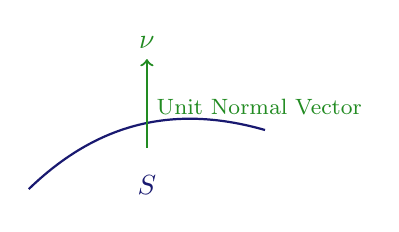
\begin{tikzpicture}[scale=1.5]
    % Surface S
    \draw[thick, MidnightBlue] (0,0) to[bend left=30] (2,0.5);
    \node[MidnightBlue, below] at (1,0.2) {$S$};
    
    % Normal Vector nu
    \draw[->, thick, ForestGreen] (1, 0.35) -- (1, 1.1) node[above] {$\nu$};
    \node[ForestGreen, right] at (1, 0.7) {\footnotesize Unit Normal Vector};
\end{tikzpicture}
\end{center}
\end{math-stroke}

% [SYSTEM] Segment complete. Please prompt "Continue" for the remainder of the segment.
% ==========================================
% SECTION 3: THE ROLE OF PROOFS IN ANALYSIS
% ==========================================
\section{The Role of Proofs in Analysis}

\begin{spoken-clean}[00:22:00 - 00:24:15]
Now I wanted to — to do a very small survey about your attitude, um, attitude towards proofs. Okay? This is important to mention that. \inlinemetanote{Moves to the right chalkboard} So I will put two columns. Column left is \qt{I find proofs} — so proofs I mean rigorous, long, very careful mathematical proofs with all details. Okay? This is mean proofs. So here I will put: I find proof, um, essential, illuminating, useful to clarify, the best part of any course. And on this column over here I will put: I find the proof innecessary, confusing, mysterious, I don't know when I have finished the proof or not, right? Because it looks like — it sounds convincing but — mysterious, no clear — no clear rules of the game.
\end{spoken-clean}

\begin{math-stroke}[Survey: Attitude Towards Proofs]
The lecturer creates a comparative table on the board to gauge student sentiment regarding formal mathematical proofs.
\begin{center}
\begin{tabular}{l | l}
\textbf{Positive / Essential} & \textbf{Negative / Challenging} \\ \hline
Essential & Innecessary \\
Illuminating & Confusing \\
Useful to clarify & Mysterious \\
The best part & No clear rules of the game
\end{tabular}
\end{center}
\end{math-stroke}

\begin{spoken-clean}[00:24:15 - 00:26:15]
And now, okay, this is extreme — I mean, I'm — I'm making all this on purpose. This is extreme, right? This is extreme. I know that any — most of you would be maybe in the middle. But I would like to know which of you lean more towards this opinion or more towards this opinion. Okay? So let's start with this one. So who is here? Who loves proofs and... okay. \inlinemetanote{Students raise hands} Okay. And here... \inlinemetanote{Students raise hands for the other column} Okay, it's interesting. So it's roughly — there are a bit more people that love proofs, but — but okay. So there is no correct answer, right? Uh, so I would be — well, depending on where — in between.
\end{spoken-clean}

\begin{spoken-clean}[00:26:15 - 00:28:30]
So why — why am I asking this? So does it coin — is it — does it have some correlation with physicists and mathematicians or not? Sometimes. What do you think? It — it could make sense, not always. There are physicists that... but — it could make sense. So I think that, um, about this discussion of proofs, I wanted to — to use ten minutes today to tell you two things. First, why I believe — many people can have many answers — but why I believe that the proofs are important and what will we test in this course, right? Because it's — it's a bit correlated of course.

So the first thing is that in — in algebra many times you have a theorem that is very beautiful, very clean, and you can apply in many situations without modifying it, right? In analysis, we will see that, sometimes the theorem that you learned doesn't exactly apply to the situation you — you need. Then you need to know how to modify a little bit the theorem. And the only way to do that is to know the proof and then modify a — some step here and some step there.
\end{spoken-clean}

\begin{didactic-insight}[Analysis as a Malleable Tool]
The lecturer highlights a fundamental difference between Algebra and Analysis: in Analysis, theorems are often not \qt{black boxes} but templates. Understanding the proof is what grants the mathematician the flexibility to adapt a result to non-standard domains or boundary conditions.
\end{didactic-insight}

\begin{spoken-clean}[00:28:30 - 00:31:17]
Also, many times the proof contains the ideas on why the theorem is true, right? The theorem is a bunch of symbols as we wrote there sometimes or statements, but it's not very illuminating. It's okay to know that a fact is true, but when you know a bit why, it's — it's — it's more useful many times, right? Being able to export and to use in situations that are new and also, um, understanding better, meaning being able also sometimes to remember the — the theorem. Because if you — if you get quick at remembering proofs and arguments, sometimes you don't remember all the assumptions of a theorem and you can figure — you can figure them out just by — by repeating the proof in — in your mind, right?

This doesn't mean that you need to learn the proof in all the details all the time. It's very important — so that the proof is useful and illuminating and so on — it's very important that when you have this super long proof, you extract the main ideas of the proof. A very short — so you need to have several levels in your head. So a proof that is that long, you can remember three sentences like hints that are the key ingredients of the proof for you. And it's very good exercise to do that. Then you expand. You learn how to expand these — these summaries. Is it clear that? And how you learn how to expand? You learn how to expand, um, hints by doing exercises. That's why the exercises are important. If you become very good in solving exercises, you'll be able to compress the information very well because then you don't need to remember all the details. You just remember the highlights of the proof and then you fill the details because you are expert in doing that, right? So becoming expert in exercises is — is good to find the proof also more interesting and more useful and not that, um, much of an effort.

Now, some people that are here that find the proof confusing, mysterious, innecessary, is because sometimes the — the rules of the game and why the game is interesting is not that clear. So why when you finish a proof, why can you say that the proof is finished, right? Because the professor says so that this the proof QED? Is common sense? Um, what is — most people see that, oh, this looks like a argument that is conclusive. Most people. But not every time. And there are very subtle arguments. So that's why we need to spend sometimes a lot of time with things that seem obvious because I tell you: a continuous function crosses the zero axis at some point (Recall: Intermediate Value Theorem). Okay, of course it crosses. But — this intermediate value theorem, right? Continuous function crosses the — of course, but you need to prove it, right? And the proof cannot be just the intuition of I make a drawing... \inlinemetanote{Draws a line crossing an axis} I have the zero line, I have two points, one here, one here, I have a continuous function, so if I cannot hold the — the pen from the paper, I need to cross the line at some point. This is not a mathematical proof. But it's a correct intuition.
\end{spoken-clean}

\begin{math-stroke}[Intuition vs. Rigor]
\begin{center}
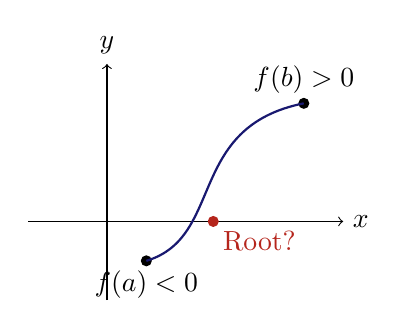
\begin{tikzpicture}[scale=1.0]
    % Axes
    \draw[->] (-1,0) -- (3,0) node[right] {$x$};
    \draw[->] (0,-1) -- (0,2) node[above] {$y$};
    
    % Points
    \fill (0.5, -0.5) circle (2pt) node[below] {$f(a) < 0$};
    \fill (2.5, 1.5) circle (2pt) node[above] {$f(b) > 0$};
    
    % Continuous curve
    \draw[thick, MidnightBlue] (0.5, -0.5) .. controls (1.5, -0.2) and (1.0, 1.2) .. (2.5, 1.5);
    
    % Intersection
    \fill[BrickRed] (1.35, 0) circle (2pt);
    \node[BrickRed, below right] at (1.35, 0) {Root?};
\end{tikzpicture}
\end{center}
\begin{explanation-of-steps}
The lecturer uses the Intermediate Value Theorem to illustrate that while geometric intuition (the \qt{pen on paper} argument) is powerful, it does not constitute a formal proof. Rigorous analysis requires proving these \qt{obvious} facts from foundational axioms.
\end{explanation-of-steps}
\end{math-stroke}

\begin{spoken-clean}[00:31:17 - 00:31:17]
Now, so what can help with this? I think that something that can help with this, with the rules of what is a proof and what is not a proof... \inlinemetanote{Turns on the projector} Now we will need to turn on the projector again. Okay. Let me see. \inlinemetanote{Projector starts up} Hmm. Okay. So if someone is interested, you can go — you can Google, let's see, Google... you can Google, uh, Natural Number Game. \inlinemetanote{Lecturer searches for the game on Google} This is a serious stuff. I mean, I'm — I'm not — this is a very serious stuff. It's difficult. I mean, I know that there are some cartoons, but this is — is a serious difficult game. So — so it's — so this is a — so one — one argument and — and now seriously, in the light of artificial intelligence and — and all what is going on. So one argument that is very interesting about proofs is that — maybe some of you didn't realize — but a proof is computable. So if a proof is correct or not can be computed. That's why it's not an opinion, right? You can — there are several computation languages for... \textit{[Audio cuts off abruptly]}
\end{spoken-clean}

\begin{meta-note}[Projected Content: The Natural Number Game]
The lecturer shows the \qt{Natural Number Game} website, an interactive tool for learning formal proof verification using the Lean proof assistant. The interface shows a progression of \qt{worlds} representing different mathematical concepts.
\end{meta-note}

\begin{math-stroke}[The Structure of Formal Proofs (Lean)]
\begin{center}
\begin{tikzpicture}[node distance=1.5cm, every node/.style={draw, rounded corners, fill=gray!10, font=\footnotesize}]
    % Nodes
    \node (Tutorial) {Tutorial World};
    \node (Addition) [below=of Tutorial] {Addition World};
    \node (Multiplication) [below left=of Addition] {Multiplication World};
    \node (Power) [below right=of Addition] {Power World};
    \node (Function) [below=of Multiplication] {Function World};
    \node (Proposition) [below=of Power] {Proposition World};
    \node (AdvAdd) [below=of Function] {Advanced Addition World};
    \node (AdvMult) [below=of Proposition] {Advanced Multiplication World};
    \node (Inequality) [below=of AdvAdd] {Inequality World};

    % Connections
    \draw[->] (Tutorial) -- (Addition);
    \draw[->] (Addition) -- (Multiplication);
    \draw[->] (Addition) -- (Power);
    \draw[->] (Multiplication) -- (Function);
    \draw[->] (Power) -- (Proposition);
    \draw[->] (Function) -- (AdvAdd);
    \draw[->] (Proposition) -- (AdvMult);
    \draw[->] (AdvAdd) -- (Inequality);
\end{tikzpicture}
\end{center}
\end{math-stroke}

% [SYSTEM] Video complete.

% --- TEIL 2 ---
\begin{spoken-clean}[00:00:00 - 00:01:56]
...people that find the proof confusing, mysterious, innecessary, is because sometimes the --- the rules of the game and why the game is interesting is not that clear. So, why when you finish a proof, why can you say that the proof is finished, right? Because the professor says so that this is the proof Q.E.D.? Is common sense? Um, what is --- most people see that, oh, this looks like a argument that is conclusive. Most people. But not every time. And there are very subtle arguments. So, that's why we need to spend sometimes a lot of time with things that seem obvious because I tell you: a continuous function crosses the zero axis at some point (Recall: Intermediate Value Theorem). Okay, of course it crosses. But --- this intermediate value theorem, right? Continuous function crosses the --- of course, but you need to prove it, right? And the proof cannot be just the intuition of I make a drawing --- I have the zero line, I have two points, one here, one here, I have a continuous function, so if I cannot hold the --- the pen from the paper, I need to cross the line at some point. This is not a mathematical proof. But it's a correct intuition. Now, so what can help with this? I think that something that can help with this, with the rules of what is a proof and what is not a proof... \inlinemetanote{The lecturer turns on the projector and searches on Google} Now we will need to turn on the projector again. Okay. Let me see. Um. Okay. So, if someone is interested, you can go --- you can Google, let's see, Google... you can Google, uh, Natural Number Game. \inlinemetanote{The lecturer navigates to the Natural Number Game website}
\end{spoken-clean}

\begin{meta-note}[Projected Content: Lean Game Server]
The lecturer displays the \qt{Lean Game Server} website, specifically the \qt{Natural Number Game}. The site is described as a repository of learning games for the proof assistant Lean (Lean 4) and the mathematical library \qt{mathlib}. Other games shown include \qt{Relativity}, \qt{Field Theory}, \qt{Thermodynamics}, and \qt{Real Analysis, The Game}.
\end{meta-note}

\begin{spoken-clean}[00:01:56 - 00:04:08]
So, if someone is interested, you can go --- you can Google, let's see, Google... you can Google, uh, Natural Number Game. Is --- this is a serious stuff. I mean, I'm --- I'm not --- this is a very serious stuff. It's difficult. I mean, I know that there are some cartoons, but this is --- is a serious difficult game. So --- so it's --- so this is a --- so one --- one argument and --- and now seriously, in the light of artificial intelligence and --- and all what is going on. So, one argument that is very interesting about proofs is that --- maybe some of you didn't realize --- but a proof is computable. So, if a proof is correct or not can be computed. That's why it's not an opinion, right? You can --- there are several computation languages for proofs, one of the most famous is this Lean, where you can write the --- the proof in the language. It's very tedious to write the proof in the language, but now there are tools that help you. And now the --- it's like a computer program. If the program compiles, the proof is correct up to the axioms. You provide the axioms, you provide the reasoning, and if the program compiles, it's --- proof is correct. And if it doesn't compile, it doesn't mean that it's not correct. It means that you need to put more details. Maybe it's not correct, maybe yes, but it's not detailed enough. Right? So, first argument is that, um, so --- or some important argument is that proof are computable, this means that this ends all the discussion. If I wrote a proof, it's true, that's it. End of the discussion. Okay? Which is interesting. So, it --- it doesn't matter if Donald Trump says that the proof --- the fundamental theorem --- I mean, no, he can say whatever he wants, but the theorem will be true, okay? That nowadays is --- this is an interesting aspect.
\end{spoken-clean}

\begin{didactic-insight}[AI and the Verifiability of Proofs]
The lecturer uses the emergence of proof assistants like Lean to ground the concept of mathematical truth. By framing a proof as a \qt{computable} object rather than a matter of opinion, he highlights the absolute rigor required in Analysis. This serves as a meta-commentary on the reliability of AI models (like ChatGPT or Gemini), which may \qt{hallucinate} plausible-sounding but logically flawed arguments, whereas a compiled Lean proof is objectively verified.
\end{didactic-insight}

\begin{spoken-clean}[00:04:08 - 00:08:20]
This also an interesting aspect for these guys, right? \inlinemetanote{Points at the ChatGPT and Gemini tabs on his browser} Right? So, I --- I had on purpose the --- the ChatGPT or the Gemini or whatever. So, you are using those, right? You are using these --- I know that some people tell you \qt{don't use that} --- well, I know you are using those. Um, and I think it's --- I think you are --- you --- you know much better how to use than --- than people think. Um, so --- but you see, these guys still, especially with more advanced proofs, hallucinate. And say things sometimes that are wrong. And then knowing how to spot this is another motivation. Knowing how to spot wrong arguments and --- and being careful with correct and incorrect arguments --- um, is a good motivation to learn how to do correct proofs. Okay? And you can train by doing exercises, and if you are not sure, if you are --- now I --- I put it down. But if you are not sure what are the rules of the game, what is a proof, what is not a proof, try to --- I know it's difficult, try to go to the Natural Number Game and play a bit, and you will see what is a fully rigorous proof up to --- up to the end. And why we don't do this all the time. Because now --- the next thing I wanted to tell you is in Analysis 2, the pace will be quicker than in Analysis 1. We'll start roughly at the same pace, do --- doing many details, and then we will go a bit faster. What does it mean faster? That I will not be as detailed. You see? Some things is \qt{because this and that, then this follows}. And then you --- if you don't see that this follows, if many don't see, you ask question: \qt{Wow, uh, why this follows? I don't see --- we don't see}. Then we can provide details. But we will not be able to stop all the time to provide details because some of the arguments you already know how to do them. The Analysis 1 arguments, I will say \qt{okay, this is like in Analysis 1}, right? So, the pace is quicker and quicker. And the more you advance in your studies, it will be quicker. This doesn't mean that you can be okay with not --- uh, understanding, right? You need to --- if some statement you don't know how to prove, you can try by yourself, you can ask your peers, you can unfold everything. And this is a very good exercise. So, you need to do your exercises, you need to try to understand all the steps of the proof, meaning that ideally you should be able with time and --- and effort to --- to go back to the axioms, right? You don't need to do every time. You --- you just need to --- to be --- to know that you are able to. Okay? And then you are okay. So, if you can do this with --- with most --- proofs, um, it --- it means that you are following very well the course. Okay?
\end{spoken-clean}

\begin{spoken-clean}[00:08:20 - 00:10:30]
Is there something else I wanted to tell you before we start with the lecture? I don't think so. So, we have roughly ten minutes before the pause. I will start with the proper --- lecture --- the second half. And then --- uh, let me ask you, do you have some questions about what I said in this first part? A bit the plan of the course, how to be successful in the course, what do we expect from you? I --- now I have the impression that I said many things and maybe --- uh, I will need to insist --- uh, later on and come back to the objectives. Let me summarize if --- if there are no questions let me summarize in three points what are the --- a bit the main learning goals. Okay? So, maybe point number one that is very relevant to both physics and --- physicists and mathematicians is being able to do computations. Computations. Computations means --- um, advanced computations. Compute the --- the solution of some O.D.E., right? Several variable stuff. A computation can be compute some integral. Why the --- the area of the sphere is --- whatever, $4\pi$ or of the radius one, $4\pi r^2$? You need to be able to compute that integrals and --- with a numeric --- so with a --- um, --- with a concrete output like a numeric value. This --- this could be a concrete goal. Then you need to be able to follow proofs. Follow the --- the logic. And this you train with exercises, that some of them are computation --- also the computations, but some of them are more computation, some of them are more theoretical. And also you can train with the lecture notes. Whenever you don't understand a passage of the lecture notes, as I said before, you train --- train to fill out details. If you cannot, no problem, you ask, you ask your peers, then you ask me, and is a good exercise. Right? So, you have plenty of material to --- of material to train.
\end{spoken-clean}

% [SYSTEM] Segment complete. Please prompt "Continue" for the remainder of the segment.
\begin{spoken-clean}[00:10:30 - 00:11:36]
And essentially these are the two --- the two main legs: so computation and proofs. And then the third leg that I will introduce a bit is --- a bit assessing if a proof is correct. This is something we didn't test in the past, but now it's becoming more and more important. Okay? So, some type of exercise that I will try to introduce at some point is giving you some proof with a flaw argument. Sometimes I make mistakes, so then it's good because you can practice this and then you see... but I will try to make less mistakes. And then if I would then do some proofs with incorrect arguments on purpose and then you can spot \qt{ah, this subtlety you --- we didn't get it right} or here --- here the ChatGPT made a hallucination, okay? It's getting more and more harder and harder to get these models to hallucinate, but still in Analysis 2 it's --- is harder now. But --- but then we will put trickier questions. Um. Okay. So, it's five minutes. Do you have any question, someone? Ah, there? Is there a question? Yeah. Okay. Thank you. Sorry, I cannot see very well so...
\end{spoken-clean}

\begin{student-question}[Rigor in Tests]
I wanted to ask how rigorous do the proofs have to be in the test? Do we have to do them like the Analysis 1 test where we have --- we don't have to write down the axioms every time, or we just mention the most important theorem, or do we have to do very rigorous proofs?
\end{student-question}

\begin{spoken-clean}[continued]
Let me --- let me put the question about --- about --- let me put the question a bit different. The proof are always very rigorous. The only thing that they don't need to be as detailed as. You see? You can do some claims and you don't need to justify to the smallest detail every single claim. In Analysis 1, you see the difference of the theorem, it's clear.
\end{spoken-clean}

\begin{meta-note}[Blackboard Transition]
The lecturer erases the left and center chalkboards to summarize the transition from Analysis I to Analysis II.
\end{meta-note}

\begin{spoken-clean}[00:12:33 - 00:13:17]
So, what would be a --- a proof of this? So, how would you summarize in a sentence a proof of --- of this equation over here? Let's try this. \inlinemetanote{Points at the FTC on the board} Yeah. Fundamental Theorem of Calculus. \inlinemetanote{Starts writing on the board}
\end{spoken-clean}

\begin{math-stroke}[The Fundamental Theorem of Calculus vs. Divergence Theorem]
The lecturer restates the central comparison between the two courses:
\begin{itemize}
    \item \textbf{Analysis 1:} Calculus of one variable.
    \[ \text{FTC} \qquad \int_{a}^{b} f'(x) \, dx = f(b) - f(a) \]
    \item \textbf{Analysis 2:} Calculus in $\ge 2$ variables.
    \[ \text{Gauss/Divergence} \qquad \int_{\Omega} \sum_{i=1}^n \frac{\partial f_i}{\partial x_i} \, dx = \int_{S} f \cdot \nu \, dS \]
\end{itemize}
\end{math-stroke}

\begin{spoken-clean}[00:13:17 - 00:15:18]
So, anyone --- someone want to tell me one sentence that kind of explains the idea of the proof of that? \inlinemetanote{Points at the FTC}
\end{spoken-clean}

\begin{student-question}[Student Answer]
We can show that the derivative of the primitive converges to the actual value of the function at the --- I think it was $a$ or no, $b$.
\end{student-question}

\begin{spoken-clean}[continued]
The derivative of the --- yeah. So, the derivative with respect to this --- this value, right? Yeah, this is a good --- a good answer. So, if --- so everyone has --- this is what I was telling you about before. So, when you see a --- something like this, the first time you see, you see all the proof, and then there --- there needs to be something that you remember. That is some summary of the proof that for each person might be a bit different. There are also several ways to do the proof. And then with this, you are able to reconstruct the details. You want to know what --- what I remember when I see this? I see --- I always remember the \qt{telescopic sum}. Do you know what is a telescopic sum, right? So, when I see this, I see --- I see that. Right? I see... let me put it there.
\end{spoken-clean}

\begin{didactic-insight}[The Telescopic Sum Analogy]
The lecturer provides a powerful mental anchor for the Fundamental Theorem of Calculus: the telescopic sum. By viewing the integral as a sum of infinitesimal increments where internal terms cancel out, leaving only the boundary values, the student gains a structural intuition that carries over to the Divergence Theorem in higher dimensions.
\end{didactic-insight}

\begin{math-stroke}[Intuition: The Telescopic Sum]
The proof of the FTC can be visualized by partitioning the interval $[a, b]$ into $N$ small sub-intervals:
\begin{center}
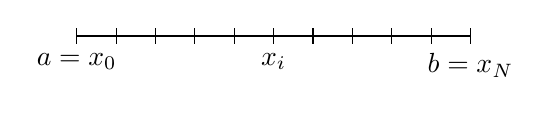
\begin{tikzpicture}
    \draw[thick] (0,0) -- (5,0);
    \foreach \x in {0, 0.5, 1, 1.5, 2, 2.5, 3, 3.5, 4, 4.5, 5}
        \draw (\x, 0.1) -- (\x, -0.1);
    \node[below] at (0, -0.1) {$a = x_0$};
    \node[below] at (5, -0.1) {$b = x_N$};
    \node[below] at (2.5, -0.1) {$x_i$};
\end{tikzpicture}
\end{center}
The difference $f(b) - f(a)$ is expanded as a sum of increments:
\begin{align*}
f(b) - f(a) &= f(x_N) - f(x_0) \\
&= \underbrace{(f(x_N) - f(x_{N-1})) + (f(x_{N-1}) - f(x_{N-2})) + \dots + (f(x_1) - f(x_0))}_{\text{Telescopic Sum}} \\
&= \sum_{i=1}^N \big( f(x_i) - f(x_{i-1}) \big)
\end{align*}
\begin{explanation-of-steps}
By multiplying and dividing each term by the step size $h = x_i - x_{i-1}$, each increment $\frac{f(x_i) - f(x_{i-1})}{h}$ approximates the derivative $f'(x_i)$. In the limit as $h \to 0$, this sum becomes the Riemann integral $\int_a^b f'(x) \, dx$.
\end{explanation-of-steps}
\end{math-stroke}

\begin{spoken-clean}[00:15:18 - 00:17:15]
So, you are unfolding this sum. Now, if you call the distance between these two consecutive points $h$, you multiply and divide by $h$, right? And each of these pieces is approximately the derivative. End of the proof. Okay? I will not go at this speed. But this is a way to remember the proof. And you need to find your own way in each proof. And then it's not that hard to remember them. Okay, so it's nine. We do the 15 minutes pose and then we start with the proper lecture. \inlinemetanote{The lecturer takes a break. The video resumes with the lecturer at the board} So, I will --- I will do my best, I will do my best to respect the schedule and the times, but please --- uh, I would ask you to do also your best to respect the 15 minutes break and be here 30 seconds before the bell --- rings and so on. Because otherwise we lost two minutes that of course are not subtracted from the exam, it just that I rush some proof, right? So, it's --- is in your interest to be on time.
\end{spoken-clean}

% ==========================================
% SECTION 4: THE SPACE R^n
% ==========================================
\section{The Space \texorpdfstring{$\mathbb{R}^n$}{Rn}}

\begin{spoken-clean}[00:17:15 - 00:19:02]
So, $\mathbb{R}^n$ we said before is the set of $n$-tuples of real numbers, right? \inlinemetanote{Writes on the board} And we will be concerned with $\mathbb{R}^n$, $n$ in $\mathbb{N}$ is the dimension of the space. Can you see from up there this? Yeah? You have very good eyes because I could not see anything. Okay. Now, $\mathbb{R}^n$ by itself --- well, --- just vectors of --- of numbers of real numbers is not --- that interesting, we will need to add some extra structure. So, what is the Euclidean --- Euclidean structure? You already know, I think, but we will say again.
\end{spoken-clean}

\begin{math-stroke}[Definition of \texorpdfstring{$\mathbb{R}^n$}{Rn}]
\begin{definition}[The Space $\mathbb{R}^n$]
The space $\mathbb{R}^n$ is the set of all $n$-tuples of real numbers:
\[ \mathbb{R}^n = \{ x = (x_1, \dots, x_n) \mid x_i \in \mathbb{R} \} \]
The natural number $n \in \mathbb{N}$ denotes the \emph{dimension} of the space.
\end{definition}
\end{math-stroke}

\begin{spoken-clean}[00:19:02 - 00:21:18]
So, in $\mathbb{R}^n$ what can we do? We can measure --- we can, well, sum vectors, right? \inlinemetanote{Writes the sum formula} We can multiply --- this is like linear algebra. If $\lambda$ is a real, we can multiply by a --- a scalar. This is a scalar, a real number. So, $\lambda x_1, \dots, \lambda x_n$. You know that from linear algebra very well. And then we can also measure the Euclidean structure means that we can also measure distances between points, right? So, we have the norm, the Euclidean norm. \inlinemetanote{Writes the norm formula}
\end{spoken-clean}

\begin{math-stroke}[Vector Space Structure of \texorpdfstring{$\mathbb{R}^n$}{Rn}]
The space $\mathbb{R}^n$ is equipped with the standard operations of a vector space:
\begin{description}
    \item[Vector Addition:] For $x, y \in \mathbb{R}^n$:
    \[ x + y = (x_1 + y_1, \dots, x_n + y_n) \]
    \item[Scalar Multiplication:] For $x \in \mathbb{R}^n$ and $\lambda \in \mathbb{R}$:
    \[ \lambda x = (\lambda x_1, \dots, \lambda x_n) \]
\end{description}
\end{math-stroke}

% [SYSTEM] Segment complete. Please prompt "Continue" for the remainder of the segment.
\begin{spoken-clean}[00:21:18 - 00:22:37]
So, first the norm, the Euclidean norm of a vector $x$ is the root, the square root of the square --- the sum of the squares of the components. $x_1^2$ to --- $x_n^2$. Right? \inlinemetanote{Writes the formula on the board} This is the length of the vector. So, in the plane, let's say... \inlinemetanote{Draws a 2D coordinate system} Let's say this is $x_1$ and this is $x_2$, this is the point $x$. The length of --- of this vector $x$, the length, is $x_1^2 + x_2^2$ square root. Pythagoras. Right? Pythagoras theorem. And the same applies to every dimension.
\end{spoken-clean}

\begin{math-stroke}[The Euclidean Norm]
The Euclidean norm (or length) of a vector $x \in \mathbb{R}^n$ is defined as:
\[ \|x\| = \sqrt{\sum_{i=1}^n x_i^2} = \sqrt{x_1^2 + \dots + x_n^2} \]

\begin{center}
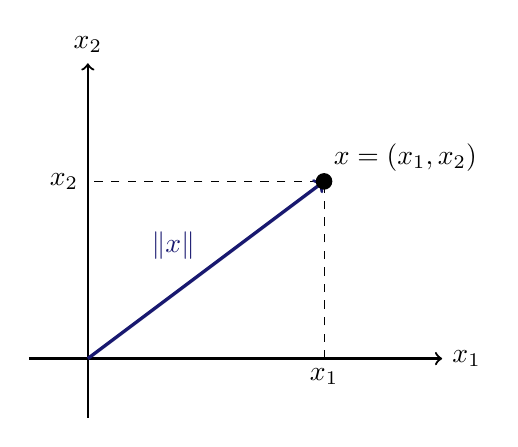
\begin{tikzpicture}[scale=1.5]
% \begin{ai-tikz-planner-invisible-content}
% 1. Background: 2D Axes.
% 2. Midground: Dashed lines to components x1, x2.
% 3. Foreground: The vector x and its label.
% \end{ai-tikz-planner-invisible-content}
    % Axes
    \draw[->, thick] (-0.5,0) -- (3,0) node[right] {$x_1$};
    \draw[->, thick] (0,-0.5) -- (0,2.5) node[above] {$x_2$};

    % Components
    \draw[dashed] (2,0) -- (2,1.5) -- (0,1.5);
    \node[below] at (2,0) {$x_1$};
    \node[left] at (0,1.5) {$x_2$};

    % Vector
    \draw[->, very thick, MidnightBlue] (0,0) -- (2,1.5) node[midway, above left] {$\|x\|$};
    \fill (2,1.5) circle (2pt) node[above right] {$x = (x_1, x_2)$};
\end{tikzpicture}
\end{center}

\begin{explanation-of-steps}
The Euclidean norm is a direct generalization of the Pythagorean theorem to $n$ dimensions, representing the straight-line distance from the origin to the point $x$.
\end{explanation-of-steps}
\end{math-stroke}

\begin{spoken-clean}[00:22:37 - 00:24:42]
Okay. And we can also measure scalar products or --- inner products that have, you know, maybe that they have to do with angles, right? The scalar products. So, we will use these notations: $x \cdot y$ or sometimes this also, $\langle x, y \rangle$. Both are fine. \inlinemetanote{Writes the summation formula} This should not be too surprising. Scalar product. And then I said the norm of a vector, that is the length of the vector, and then the distance between points. What is the distance between points? If I take two points here... \inlinemetanote{Draws two points $x$ and $y$ in space} One point $x$ and one point $y$ over here, the distance between the two points is the length of the vector that joins them, no? The distance between $x$ and $y$ is the length of the vector that joins them. This a definition. This is the Euclidean distance.
\end{spoken-clean}

\begin{math-stroke}[Scalar Product and Distance]
The space is further structured by the \emph{scalar product} (or inner product):
\begin{color-box}{BrickRed}[Scalar Product]
\[ x \cdot y = \langle x, y \rangle = \sum_{i=1}^n x_i y_i \]
\end{color-box}

The \emph{Euclidean distance} between two points $x, y \in \mathbb{R}^n$ is defined as the norm of their difference:
\begin{equation} \label{eq:distance_def}
d(x, y) = \|y - x\| = \sqrt{\sum_{i=1}^n (y_i - x_i)^2}
\end{equation}

\begin{center}
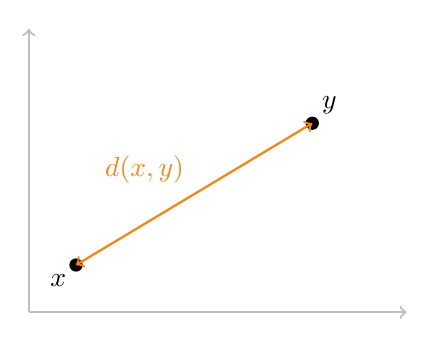
\begin{tikzpicture}[scale=1.2]
    \coordinate (X) at (0.5, 0.5);
    \coordinate (Y) at (3, 2);
    
    \draw[->, thick, gray!50] (0,0) -- (4,0);
    \draw[->, thick, gray!50] (0,0) -- (0,3);
    
    \fill (X) circle (2pt) node[below left] {$x$};
    \fill (Y) circle (2pt) node[above right] {$y$};
    
    \draw[thick, BurntOrange, <->] (X) -- (Y) node[midway, above left] {$d(x, y)$};
\end{tikzpicture}
\end{center}
\end{math-stroke}

\begin{spoken-clean}[00:24:42 - 00:26:37]
Now, the first lemma I will prove about Euclidean distance is the triangle inequality. Triangle inequality. Do you know the --- some of you know the triangle inequality? Have you seen that? Who --- how many people have not seen the triangle inequality? Ah, you all know the triangle inequality. Okay, then I will be quick on that. So, the triangle inequality says this: for all $x, y, z$ in $\mathbb{R}^n$, for all --- triples of vectors, if I do $z - x$, the length of this is less than the length of going from $x$ to $y$ plus the length of going from $y$ to $z$. Right? \inlinemetanote{Writes the inequality on the board} Maybe you have seen the triangle inequality with the absolute value? Have --- but you have also seen that one, with the modulus, with the length. Right? So, what this says is that whenever you have three points $x, y, z$ in the space in any position... \inlinemetanote{Draws a triangle with vertices $x, y, z$} The length --- so the --- the distance between $x$ and $z$ is always longer than this --- the sum of these two distances. Right? Or equal. And actually it is equal when the point is aligned with the two, right? But I'm not saying this yet.
\end{spoken-clean}

\begin{math-stroke}[Lemma: The Triangle Inequality]
\begin{color-box}{black}[Triangle Inequality]
\begin{lemma}[Triangle Inequality] \label{lem:triangle_inequality}
For all $x, y, z \in \mathbb{R}^n$, the following inequality holds:
\begin{equation} \label{eq:triangle_xyz}
\|z - x\| \le \|y - x\| + \|z - y\|
\end{equation}
\end{lemma}
\end{color-box}

\begin{center}
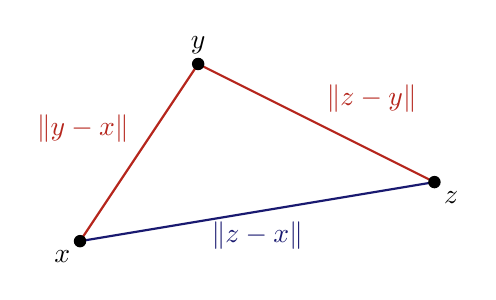
\begin{tikzpicture}[scale=1.5]
    \coordinate (X) at (0,0);
    \coordinate (Y) at (1, 1.5);
    \coordinate (Z) at (3, 0.5);
    
    \draw[thick, MidnightBlue] (X) -- (Z) node[midway, below] {$\|z - x\|$};
    \draw[thick, BrickRed] (X) -- (Y) node[midway, above left] {$\|y - x\|$};
    \draw[thick, BrickRed] (Y) -- (Z) node[midway, above right] {$\|z - y\|$};
    
    \fill (X) circle (1.5pt) node[below left] {$x$};
    \fill (Y) circle (1.5pt) node[above] {$y$};
    \fill (Z) circle (1.5pt) node[below right] {$z$};
\end{tikzpicture}
\end{center}

\begin{explanation-of-steps}
Geometrically, the triangle inequality states that the shortest path between two points is a straight line. Any detour through a third point $y$ must result in a total distance that is greater than or equal to the direct distance.
\end{explanation-of-steps}
\end{math-stroke}

\begin{spoken-clean}[00:26:37 - 00:29:18]
So, let's prove that. So, to prove that equivalently I will prove --- equivalently, I'm saying that $\|x + y\|$ is less than or equal to $\|x\| + \|y\|$. \inlinemetanote{Writes the equivalent form on the board and labels it with a red star} So, why is this equivalent to this one? Well, equivalent is means that if you know how to prove this, easily you prove that, right? Why is this equivalent to this one? Well, you see the difference of the theorem, it's clear. So, what would be a proof of this? So, you need to do this substitution. You can call $a$ the vector $y - x$, say, then $b$ is equal to $z - y$, and then automatically if you sum $a + b$ is --- is $z - x$. Right? \inlinemetanote{Writes the substitution on the board} This is like putting --- so one --- so if you want to go from here to here, you just put as he said $z$ equal to --- so you need to put here is $x + y$. Well, you need to do this substitution, this kind of substitution, and it works both ways, right? Because if you do this, you will get $a + b$ less than or equal to to that and --- and the opposite. If you --- use this inequality with this substitution, you will get that. Now, this is as detailed as I will be, again. A bit the difference between Analysis 1 and 2. If this equivalence poses some trouble, it shouldn't pose too much, but you can work a bit by yourself, is a nice exercise. Okay? And if you cannot, um, ask later.
\end{spoken-clean}

\begin{math-stroke}[Equivalence of Triangle Inequality Forms]
The statement in Equation \ref{eq:triangle_xyz} is equivalent to the following simpler form:
\begin{color-box}{black}[Equivalent Form]
\begin{equation} \label{eq:triangle_star}
\|x + y\| \le \|x\| + \|y\| \tag{\textcolor{BrickRed}{$\ast$}}
\end{equation}
\end{color-box}

\begin{proof}[Proof of Equivalence]
To see the equivalence, we perform a change of variables. Let:
\begin{align*}
a &= y - x \\
b &= z - y
\end{align*}
Summing these vectors yields:
\[ a + b = (y - x) + (z - y) = z - x \]
Substituting these into Equation \ref{eq:triangle_xyz}, we obtain:
\[ \|a + b\| \le \|a\| + \|b\| \]
which is exactly the form of Equation \ref{eq:triangle_star}. Since the mapping $(x, y, z) \mapsto (a, b)$ is surjective, the two statements are logically equivalent.
\end{proof}
\end{math-stroke}

\begin{spoken-clean}[00:29:18 - 00:31:17]
Okay, so this is the --- since we convinced ourselves that the two statements are equivalent and this is shorter, I will prove this one. So, now the goal is to prove that inequality. Okay? And now I will do it maybe in the next blackboard. \inlinemetanote{Moves to the next chalkboard} So, I start writing... let me call this inequality star. \inlinemetanote{Writes \qt{*} next to the formula} So, this what I want to show is equivalent after squaring, right? I square and I said $\|x + y\|^2$ is equal --- is less than or equal to $\|x\|^2 + \|y\|^2 + 2\|x\|\|y\|$. Right? \inlinemetanote{Writes the squared inequality} That inequality is equivalent to this one because is an inequality between positive numbers and the square --- squaring is a monotone function. This is the part that I said in words but I will not write because we are in Analysis 2. Okay? This you learned in Analysis 1. Now, once I wrote it in this form, I can develop this. What is the modulus of squared? This is equal by definition to the sum of $(x_i + y_i)^2$ between $i$ equal 1 and $n$. Right? \inlinemetanote{Writes the summation} And this is --- and this I can go --- this is equal, develop the --- now these are real numbers, so I can develop the squares. This is the sum... \textit{[Audio cuts off abruptly]}
\end{spoken-clean}

\begin{math-stroke}[Proof Strategy for the Triangle Inequality]
\begin{ai-proof-skeleton-invisible-content}
% 1. Square both sides of the inequality (*).
% 2. Expand the left side using the definition of the norm and summation.
% 3. Use the Cauchy-Schwarz inequality to bound the cross terms.
\end{ai-proof-skeleton-invisible-content}
We aim to prove Equation \ref{eq:triangle_star}. Since both sides are non-negative, it is equivalent to prove the squared version:
\[ \|x + y\|^2 \le (\|x\| + \|y\|)^2 = \|x\|^2 + \|y\|^2 + 2\|x\|\|y\| \]
Expanding the left-hand side using the definition of the Euclidean norm:
\begin{align*}
\|x + y\|^2 &= \sum_{i=1}^n (x_i + y_i)^2 \\
&= \sum_{i=1}^n (x_i^2 + 2x_i y_i + y_i^2) \\
&= \sum_{i=1}^n x_i^2 + 2\sum_{i=1}^n x_i y_i + \sum_{i=1}^n y_i^2 \\
&= \|x\|^2 + 2(x \cdot y) + \|y\|^2
\end{align*}
\textit{[Audio cuts off abruptly]}
\end{math-stroke}

% [SYSTEM] Video complete.

% --- TEIL 3 ---
% ==========================================
% SECTION 4: THE SPACE R^n (CONTINUED)
% ==========================================

\begin{spoken-clean}[00:00:00 - 00:01:24]
Right? Because if you do this (i.e., the substitution $a = y - x$ and $b = z - y$), you will get $a + b$ less than or equal to to that and --- and the opposite. If you, uh, use this inequality with this substitution, you will get that. Now, this is as detailed as I will be, again. A bit the difference between Analysis 1 and 2. If this equivalence poses some trouble, it shouldn't pose too much, but you can work a bit by yourself, is a nice exercise. Okay? And if you cannot, um, ask later.

Okay, so this is the --- since we convinced ourselves that the two statements are equivalent and this is shorter, I will prove this one (i.e., Equation \ref{eq:triangle_star}). So, now the goal is to prove that inequality. Okay? And now I will do it maybe in the next blackboard. \inlinemetanote{Moves to the center-left chalkboard} So, I start writing... let me call this inequality star. \inlinemetanote{Writes \qt{*} next to the formula} So, this what I want to show is equivalent after squaring, right? I square and I said...
\end{spoken-clean}

\begin{math-stroke}[Proof of the Triangle Inequality (Initial Attempt)]
\begin{ai-proof-skeleton-invisible-content}
% 1. Goal: Prove ||x + y|| <= ||x|| + ||y||.
% 2. Method: Square both sides and expand.
% 3. Note: The lecturer initially writes x - y on the board.
\end{ai-proof-skeleton-invisible-content}
To prove the triangle inequality, we consider the squared norm of the sum of two vectors. \inlinemetanote{The lecturer initially writes the formula for the difference $x - y$ on the board}
\begin{equation} \label{eq:triangle_sq_wrong}
\|x - y\|^2 \le \|x\|^2 + \|y\|^2 + 2\|x\|\|y\| \quad \textcolor{red}{\text{(Incorrect notation)}}
\end{equation}
Expanding the left-hand side by the definition of the Euclidean norm:
\[
\sum_{i=1}^n (x_i - y_i)^2 = \dots
\]
\end{math-stroke}

\begin{spoken-clean}[00:01:24 - 00:02:15]
...I square and I said $x$ minus $y$ squared (i.e., actually $x + y$ as intended for the proof) is equal --- is less than or equal to $x$ squared plus $y$ squared plus two times the product of the modulus. Right? That inequality is equivalent to this one because is an inequality between positive numbers and the square --- squaring is a monotone function. This is the part that I said in words but I will not write because we are in Analysis 2. Okay? This you learned in Analysis 1. Now, once I wrote it in this form, I can develop this. What is the modulus of squared? This is equal by definition to the sum of $x_i$ minus $y_i$ squared between $i$ equal 1 and $n$. Right?
\end{spoken-clean}

\begin{student-question}[Student Spotting the Sign Error]
Um, shouldn't it be $x + y$ at the beginning of the proof? There \inlinemetanote{points at the board}.
\end{student-question}

\begin{spoken-clean}[continued]
Ah, yes. Actually is the same but, yeah, now that you say it, is better. So, you can put $x + y$ is --- is equivalent to put $x + y$ and $x - y$ but --- but to match this inequality (i.e., Equation \ref{eq:triangle_star}) otherwise it would be with a minus. But all the proof you can do with the plus and with the minus but --- okay, then here will be a plus. Thank you. Thank you for the --- nice. \inlinemetanote{Corrects the board}
\end{spoken-clean}

\begin{math-stroke}[Proof of the Triangle Inequality (Corrected)]
\begin{proof}
We aim to prove Equation \ref{eq:triangle_star}: $\|x + y\| \le \|x\| + \|y\|$. Since both sides are non-negative, this is equivalent to proving:
\begin{equation} \label{eq:triangle_sq_correct}
\|x + y\|^2 \le (\|x\| + \|y\|)^2 = \|x\|^2 + \|y\|^2 + 2\|x\|\|y\|
\end{equation}
Expanding the left-hand side using the definition of the Euclidean norm and the properties of real numbers:
\begin{align*}
\|x + y\|^2 &= \sum_{i=1}^n (x_i + y_i)^2 \\
&= \sum_{i=1}^n (x_i^2 + y_i^2 + 2x_i y_i) \\
&= \underbrace{\sum_{i=1}^n x_i^2}_{\|x\|^2} + \underbrace{\sum_{i=1}^n y_i^2}_{\|y\|^2} + 2\underbrace{\sum_{i=1}^n x_i y_i}_{x \cdot y} \\
&= \|x\|^2 + \|y\|^2 + 2(x \cdot y)
\end{align*}
Substituting this back into Equation \ref{eq:triangle_sq_correct}, we see that the inequality holds if and only if:
\[
\|x\|^2 + \|y\|^2 + 2(x \cdot y) \le \|x\|^2 + \|y\|^2 + 2\|x\|\|y\|
\]
Canceling the common terms $\|x\|^2$ and $\|y\|^2$ and dividing by 2, we find that the triangle inequality is equivalent to the following condition:
\begin{equation} \label{eq:cs_goal}
x \cdot y \le \|x\|\|y\|
\end{equation}
\end{proof}
\end{math-stroke}

\begin{spoken-clean}[00:03:28 - 00:05:50]
Right? Which is equal to the modulus of $x$ squared plus the modulus of $y$ squared. This is the modulus of $x$ squared when you sum over $n$, over $i$. This is the modulus of $y$ squared and this is two times the scalar product. Right? So, I want to prove --- this is a bit like a snake, but these are equalities. This is equal to this, is equal to this. So, what I'm left with --- I'm left with proving that this thing is less than or equal to this thing. And you see here, this --- this I can simplify, right? I can simplify because it's both sides. So, what I want to show is that two $x$ dot $y$ is less than or equal than the product of the modulus. Right? So, after this calculation, what I want to prove is equivalent to this. Let me simplify also the two. Is equivalent to this (i.e., Equation \ref{eq:cs_goal}).

And this is an inequality that is famous. Now I will prove it in case you don't know. But this is the Cauchy-Schwarz inequality. Okay? And this is true, this inequality is true because is the Cauchy-Schwarz. \inlinemetanote{Writes \qt{true Cauchy-Schwarz inequality} on the board} And now, in case just to warm up and in case you didn't remember or you never saw the proof of the Cauchy-Schwarz inequality, I will prove the Cauchy-Schwarz inequality, right? So, if I can prove this inequality, you see that the proof of the triangle inequality is done, is concluded. I'm just left with proving this inequality that I told you is called the Cauchy-Schwarz inequality. So, let me do this in a --- so I will put a square that means end of the proof but up to this ingredient that I will prove next.
\end{spoken-clean}

\begin{nice-box}[Lemma: Cauchy-Schwarz Inequality]
\begin{lemma}[Cauchy-Schwarz Inequality] \label{lem:cauchy_schwarz}
For all $x, y \in \mathbb{R}^n$, the following inequality holds:
\begin{equation} \label{eq:cauchy_schwarz}
x \cdot y \le \|x\|\|y\|
\end{equation}
\end{lemma}
\end{nice-box}

\begin{math-stroke}[Proof of the Cauchy-Schwarz Inequality]
\begin{proof}
The first observation is that if either $x = 0$ or $y = 0$, the inequality is trivially satisfied as $0 \le 0$. Therefore, we assume without loss of generality (WLOG) that both $x \neq 0$ and $y \neq 0$.

Recall the definition of the scalar product:
\[ x \cdot y = \sum_{i=1}^n x_i y_i \]
We introduce a parameter $\lambda > 0$. For any such $\lambda$, we can multiply and divide each term by $\lambda$:
\[ 2(x \cdot y) = \sum_{i=1}^n 2(x_i \lambda) \left( \frac{y_i}{\lambda} \right) \]
Using the elementary inequality for real numbers $2ab \le a^2 + b^2$ (which follows from $(a-b)^2 \ge 0$), we apply this to each term in the sum:
\begin{align*}
2(x \cdot y) &\le \sum_{i=1}^n \left( (x_i \lambda)^2 + \left( \frac{y_i}{\lambda} \right)^2 \right) \\
&= \lambda^2 \sum_{i=1}^n x_i^2 + \frac{1}{\lambda^2} \sum_{i=1}^n y_i^2 \\
&= \lambda^2 \|x\|^2 + \frac{1}{\lambda^2} \|y\|^2
\end{align*}
This inequality holds for any $\lambda > 0$. To obtain the tightest bound, we choose $\lambda$ such that the two terms on the right are equal. Setting $\lambda^2 \|x\|^2 = \frac{1}{\lambda^2} \|y\|^2$ yields:
\[ \lambda^2 = \frac{\|y\|}{\|x\|} \]
Substituting this optimal value of $\lambda^2$ back into the inequality:
\begin{align*}
2(x \cdot y) &\le \left( \frac{\|y\|}{\|x\|} \right) \|x\|^2 + \left( \frac{\|x\|}{\|y\|} \right) \|y\|^2 \\
&= \|y\|\|x\| + \|x\|\|y\| \\
&= 2\|x\|\|y\|
\end{align*}
Dividing by 2, we arrive at the Cauchy-Schwarz inequality:
\[ x \cdot y \le \|x\|\|y\| \]
\end{proof}
\end{math-stroke}

\begin{spoken-clean}[00:05:50 - 00:08:20]
So, now I say Lemma, Cauchy-Schwarz inequality. Well, I don't copy. Lemma, this holds. Right? Cauchy-Schwarz inequality. In the notes will be as a separate lemma. But now I don't make me copy again because I'm going to write again exactly the same. So, this inequality holds for all $x$ and $y$ in $\mathbb{R}^n$. Okay? Now, proof. In the notes I have put two proofs. There are many ways to prove this. I have put two proofs of this inequality. I will with give one, okay?

The first observation is that if either $x$ equal zero or $y$ equal zero, the inequality is --- zero less than or equal to zero, right? Because if --- if the vector is --- if the vector one of the two vectors is zero, this product is zero and the modulus of one of the two will be zero so is zero less than or equal to zero. Which is trivially true. By this observation, I can assume without loss of generality that both vectors are not zero. So, assume without loss of generality (WLOG) both $x$ and $y$ are different from zero. This we have seen many times now you are in the second semester, this \qt{assume without loss of generality} phrasing.
\end{spoken-clean}

\begin{spoken-clean}[00:08:20 - 00:10:30]
Okay, so both vectors are non-zero. Now what I will do, um, I will take --- want to prove --- I will write what is the scalar product $x$ dot $y$. This is the sum between $i$ equal 1 and $n$, I copy again, $x_i y_i$. Right? And now I will do a trick. Um, I will take for every --- for every number $\lambda$ positive, I have the right to divide and multiply by $\lambda$. I will put $\lambda$ here and $\lambda$ over here. Right? I did nothing because I multiplied and divided by $\lambda$. And now I --- I will use an $n$ times an inequality of real numbers. You know that --- or let me --- let me multiply by two here and here. And now I will use an inequality of real numbers: $2ab$ is less than or equal to $a^2 + b^2$. Which is the same as --- essentially that $(a-b)^2$ is non-negative. So, this inequality of real numbers, I will apply $n$ times to each of these two numbers. This will be the $a$ and this will be the $b$ in each case. And what do I get? And with the two, right? I get this is less than or equal than the sum $i$ equal 1 to $n$. Now, the $\lambda$, I get $\lambda^2 x_i^2$ plus $y_i^2$ over $\lambda^2$. Okay? Which is the same as $\lambda^2$ mod $x$ squared plus 1 over $\lambda^2$ mod $y$ squared. And this holds for every $\lambda$. Right? This inequality holds for every $\lambda$ positive. I didn't use anything. Now is where I use that both are --- are not zero, so I can take $\lambda$ equal --- or $\lambda^2$ equal what? $y$ divided by $x$. We take that $\lambda$ and you get $\lambda^2$ two times, you see this --- when you get the 1 over $\lambda$ exactly simplifies what you want and you get two times the product. Okay? This is the proof of the Cauchy-Schwarz and this ends the proof of the triangle inequality. Is there any question about this proof?
\end{spoken-clean}

\begin{meta-note}[Segment Transition]
The lecturer has finished the proofs of the triangle inequality and the Cauchy-Schwarz inequality. He erases the center and right chalkboards to transition to the next major topic: Metric Spaces.
\end{meta-note}

% ==========================================
% SECTION 5: METRIC SPACES
% ==========================================
\section{Metric Spaces}

\begin{spoken-clean}[00:10:30 - 00:12:50]
This is the structure $\mathbb{R}^n$ with this structure of the scalar product, the length, is the main structure we will use in the proof to do analysis. But there are --- now we need to understand convergence sequences in $\mathbb{R}^n$, we need to understand Cauchy sequences and all these things that you understood in $\mathbb{R}$. Everything --- a bit the summary --- everything that you learned how to do in $\mathbb{R}$, now we need to learn how to do in $\mathbb{R}^n$. But --- to make it more efficient, we will learn all these concepts in a more general, um, --- from a more general viewpoint, that is from the viewpoint of metric spaces. Right? So that later when you modify --- so when you go to other --- courses or in this course later on we will have different metric spaces, I don't need to redefine all the time what convergence means and so on.

Now, I'm --- I need to warn you, especially for the --- well, I don't know if especially for the physicists, but this --- this --- now will get a bit more abstract. But bear with --- then we will come --- this will be for a --- for a couple of weeks or so. Later we will come back to $\mathbb{R}^n$, everything $\mathbb{R}^n$. But this is metric spaces topology is more axiomatic, more abstract. It's good to practice proofs because here you need to use axioms. You cannot use your intuitions all the time. You need to go back to the axioms of what is a metric space that I will tell you now and do the proofs. Sometimes working like mathematicians in more abstract viewpoint with few --- fewer axioms, um, is also easier. Well, depends, right? But it's easier because if you have less axioms --- now in $\mathbb{R}^n$ we have many axioms, we have the axiom of the supremum for each coordinate, you have many things. Now in the metric space, I will introduce three axioms. Just three. And then all the proofs need to use these three axioms. So, you don't need to think too much what are --- it's like --- like playing chess, I say sometimes, like playing chess only with the rooks. So, if you play chess only and there are only the rooks, it's not that difficult than playing with many pieces, right? So, but then you need a bit more of abstraction because it's not what you are used to. So, we are going to play chess with the rooks and we will define a metric space.
\end{spoken-clean}

\begin{didactic-insight}[The \qt{Chess with Rooks} Analogy]
The lecturer uses a playful analogy to explain the pedagogical value of abstraction. By stripping away the specific properties of $\mathbb{R}^n$ and focusing on the minimal axioms of a metric space, the \qt{rules of the game} become simpler but require more rigorous adherence. This prevents students from relying on geometric intuition that might fail in more exotic spaces (like function spaces).
\end{didactic-insight}

\begin{nice-box}[Definition: Metric Space]
\begin{definition}[Metric Space] \label{def:metric_space}
A \emph{metric space} is a pair $(X, d)$, where $X$ is a non-empty set and $d$ is a mapping (called the \emph{distance} or \emph{metric}):
\[ d: X \times X \to [0, \infty) \]
that satisfies the following three axioms for all $x, y, z \in X$:
\begin{enumerate}
    \setcounter{enumi}{0} \item \emph{Definiteness:} $d(x, y) = 0 \iff x = y$.
    \setcounter{enumi}{1} \item \emph{Symmetry:} $d(x, y) = d(y, x)$.
    \setcounter{enumi}{2} \item \emph{Triangle Inequality:} $d(x, z) \le d(x, y) + d(y, z)$.
\end{enumerate}
\end{definition}

\begin{explanation-of-steps}
The lecturer notes that while he formally defines $X$ as a set, he will not be overly pedantic about the case where $X$ might be empty, as it is trivial and lacks mathematical interest for the course.
\end{explanation-of-steps}
\end{nice-box}

\begin{spoken-clean}[00:12:50 - 00:15:15]
So, we will define a metric space is a pair $(X, d)$ where $X$ is a non-empty set. Well, let's say --- this also the kind of things that I will not be that careful about. So, if the set $X$ is empty or non-empty --- I mean, this is the part that I'm sorry to say that, but who cares? Uh, if the set is --- so if someone wants to say \qt{no, because with the empty set}, okay, in the notes probably everything is okay and I say that the set of is non-empty. In the lecture I will not focus on the case that the set can be empty or not, unless it is important and --- and hides some important subtlety. So, $X$ is a set that is non-empty, but let's not put it. And $d$ --- this is the definition, sorry, this is the definition of metric space. And $d$ is a map from the product $X$ times $X$ to the non-negative real numbers that will be called the distance. This is called the distance. And this distance satisfies three axioms.

Axiom number one is that is called is definite. That is for every pair of points $x$ and $y$ in $X$, in my space, so the distance between the two points is zero if and only if the points are the same. The distance between a point and itself is zero, of course, because what sort of distance would be non-zero from a point to itself? And if the points are different, the distance will not be zero because otherwise this distance would not be able to distinguish points, right? Axiom number two: the distance is symmetric. The distance between $x$ and $y$ is the same as the distance between $y$ and $x$. Okay? This axiom is very also very reasonable for a distance. In applications, uh, this is not always true if you think of a distance like the distance of flying --- uh, with a plane between two cities. You know that when you fly to the west is usually take less time than fly to the east? No, flying to the west takes less time than flying to the east? Due to the --- to the atmospheric drift. So, it's not always true in every situation that the distance is symmetric, but in many situations it is true. And the third axiom is the triangle inequality.
\end{spoken-clean}

\begin{spoken-clean}[00:15:15 - 00:17:15]
These are the axioms of a metric space. First example --- now I will give some examples, no? First example of a metric space: the Euclidean space $\mathbb{R}^n$ with the distance the length of a vector. Is very easy that it satisfies the --- the three axioms. So, examples. $\mathbb{R}^n$ with the Euclidean distance $d_{\text{Euclidean}}$. Why do we specify both the set and the distance? Because sometimes the same set has two or more interesting distances, right? For instance, in $\mathbb{R}^2$ I can put the Euclidean distance or I can put a different distance that you can check also satisfies that is called the --- in $\mathbb{R}^2$ there is this distance, uh, the New York distance (i.e., the Manhattan distance). That is mod $x_1$ minus $y_1$ plus mod $x_2$ minus $y_2$. Right? This is called the Manhattan distance. Why? Because this is the sort of distance when you live in one of these modern American cities or --- where the streets go north to south and east to west and you want to go from point $x$ to $y$, right? Then you cannot go diagonal because you hit the buildings and then you need to go like that. And then the distance between two points is --- is this thing. Okay? And you can check very easily that this still satisfies all the axioms of the distance. Right?
\end{spoken-clean}

\begin{math-stroke}[Examples of Metrics on \texorpdfstring{$\mathbb{R}^n$}{Rn}]
\begin{enumerate}
    \setcounter{enumi}{0} \item \emph{Euclidean Metric:} The standard distance in $\mathbb{R}^n$:
    \[ d_2(x, y) = \|x - y\| = \sqrt{\sum_{i=1}^n (x_i - y_i)^2} \]
    \setcounter{enumi}{1} \item \emph{Manhattan Metric (Taxicab Metric):} Common in grid-based layouts:
    \[ d_1(x, y) = |x_1 - y_1| + |x_2 - y_2| \]
\end{enumerate}

\begin{center}
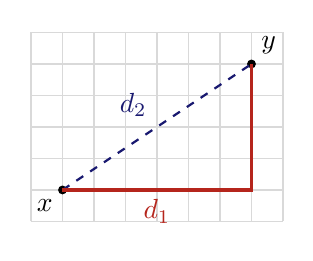
\begin{tikzpicture}[scale=0.8]
% \begin{ai-tikz-planner-invisible-content}
% 1. Background: A grid representing city blocks.
% 2. Midground: Points x and y.
% 3. Foreground: The L1 path (Manhattan) and the L2 path (Euclidean).
% \end{ai-tikz-planner-invisible-content}
    % Grid
    \draw[step=0.5, gray!30, thin] (0,0) grid (4,3);
    
    % Points
    \coordinate (X) at (0.5, 0.5);
    \coordinate (Y) at (3.5, 2.5);
    \fill (X) circle (2pt) node[below left] {$x$};
    \fill (Y) circle (2pt) node[above right] {$y$};
    
    % Euclidean Distance
    \draw[thick, MidnightBlue, dashed] (X) -- (Y) node[midway, above left] {$d_2$};
    
    % Manhattan Distance
    \draw[very thick, BrickRed] (0.5, 0.5) -- (3.5, 0.5) -- (3.5, 2.5);
    \node[BrickRed, below] at (2, 0.5) {$d_1$};
\end{tikzpicture}
\end{center}
\end{math-stroke}

\begin{spoken-clean}[00:17:15 - 00:19:15]
So, when you have a bit more abstract example, when you have any metric space and you have a subset of it, you can just restrict this distance to the --- to $Y$. So, $d$ restricted to $Y$ cross $Y$ with $Y$, this is another metric space. Right? If you take a subset of your given metric space and restrict the distance, is --- will be always a metric space. So, example, more --- this is a bit always true, a more concrete example would be if this is $\mathbb{R}^3$ with the Euclidean distance, right? And I take a subset that is the two-dimensional sphere. Let me draw it like this. $S^2$ is the set of points $x$ in $\mathbb{R}^3$ such that the length of $x$ is one. Right? This $S^2$, the sphere. Then I can see the sphere as a metric space with the Euclidean distance. So, the distance between these two points of the sphere, this one and this one say, is just you take the straight segment and measure the length. And this satisfies the axioms of the distance. Is a restriction of the Euclidean distance. You can say \qt{okay, but this distance maybe is not the best}. Because as I was saying before, if you travel by plane, this is not the distance between points. The distance between points --- a first approximation of the distance between points when you travel by plane is the geodesic distance. That is the length of the arc, the shortest arc on the surface of the earth. This is another distance. Right? Same set can have multiple meaningful distances depending on the context.
\end{spoken-clean}

\begin{math-stroke}[Subspaces and the Sphere]
\begin{ai-type-check-invisible-content}
% (X, d) is a metric space. Y \subset X.
% d|_Y is the restriction of d to Y x Y.
\end{ai-type-check-invisible-content}
Any subset $Y \subset X$ of a metric space $(X, d)$ inherits a metric structure by restricting the distance function to $Y \times Y$.

\emph{Example: The Unit Sphere $S^2 \subset \mathbb{R}^3$:}
\[ S^2 = \{ x \in \mathbb{R}^3 \mid \|x\| = 1 \} \]
The sphere can be equipped with two distinct metrics:
\begin{description}
    \item[Inherited Euclidean Metric:] The straight-line distance through the interior of the sphere.
    \item[Geodesic Metric:] The distance measured along the surface of the sphere (great-circle distance).
\end{description}

\begin{center}
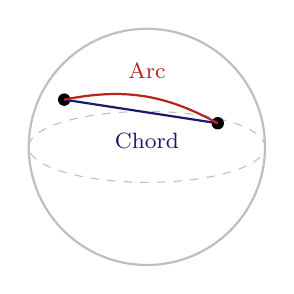
\begin{tikzpicture}[scale=1.5]
    % Sphere
    \draw[thick, gray!50] (0,0) circle (1);
    \draw[dashed, gray!50] (0,0) ellipse (1 and 0.3);
    
    % Points
    \coordinate (A) at (-0.7, 0.4);
    \coordinate (B) at (0.6, 0.2);
    \fill (A) circle (1.5pt);
    \fill (B) circle (1.5pt);
    
    % Euclidean distance (chord)
    \draw[thick, MidnightBlue] (A) -- (B);
    
    % Geodesic distance (arc)
    \draw[thick, BrickRed, bend left=20] (A) to (B);
    
    \node[MidnightBlue, below] at (0, 0.2) {\footnotesize Chord};
    \node[BrickRed, above] at (0, 0.5) {\footnotesize Arc};
\end{tikzpicture}
\end{center}
\end{math-stroke}

\begin{spoken-clean}[00:19:15 - 00:21:15]
And now maybe before --- let me do a couple more of examples. I will put it here. Maybe I need to erase something. So, one thing that can be useful when you try to do a proof in this setup that is a bit abstract of metric spaces, remember you have very few axioms you can use, but then you have less intuition. So, how you --- how can you overcome your lack of intuition? What you do is you --- you think of a specific example. Don't think of a general metric space. A general metric space means a billion of things at the same time, right? Is an abstract model of many things at the same time. Pick a concrete example. Pick the Euclidean space. Do your proof in the Euclidean space using your intuitions that you have from the space. And then try to see which axioms are you using. If you can use --- maybe you use the wrong proof and you are not using just those axioms. But then try to modify your proof using your intuition until you can do with those axioms. Okay? This can be useful. So, whenever things are abstract, don't think always in the abstract, just go to concrete examples. And this applies always because I have seen many times in more advanced courses doing examinations that you ask --- so people know the abstract theory very well and then you ask in a concrete case. \qt{So, give me the --- no, no, don't tell me the Ricci curvature on a --- no, what is in the Euclidean space?} And then people sometimes don't know how to answer. And this is a problem. So, the abstract is good but you need to know very well and think --- spend time thinking about concrete examples.

So, let me give you so that you can see also that things start to be interesting very soon. Let me give you some more interesting examples of metric space, right? Now we saw spaces of points. We can also consider spaces of functions. Now, you learned what is a continuous function. Let's say $a, b$ are two real numbers, $a < b$. And you can take $X$ the space of continuous functions from the closed interval $[a, b]$ to $\mathbb{R}$. $f$ continuous. This is a space of functions. So, one point in this space would look something like this... \inlinemetanote{Draws a curve on a coordinate system} This is one point in this space. How can we define a distance between functions? Well, in many ways. Something that is used often is the supremum distance or the maximum distance. Is the distance between $f$ and $g$ is the maximum in $[a, b]$ of the absolute value of the difference. So, you take two curves here, different, and then you look at the maximal oscillation --- so the maximum difference between the two functions. This is a distance between functions. If this is zero, the two functions are equal? Yes. Only if? Yes, is a bit more you need to reason but they are continuous so you can do that. Exercise. Does it satisfy the triangle inequality? Prove it. The symmetry is very easy that you replace $f$ and $g$ is the same because here you have the absolute value. But the triangle inequality you can prove it using the triangle inequality for the absolute value and playing with the maximum.

Another distance between functions... \inlinemetanote{Writes the integral formula} You measure the distance, you square, you integrate and you take the square root. This is another distance. Very important, the $L^2$ distance. We will not use this in a course, but you will see that you will use this later on many, many times. So, we will continue next time from --- from here.
\end{spoken-clean}

\begin{math-stroke}[Metrics on Function Spaces]
Let $X = C([a, b], \mathbb{R})$ be the set of all continuous functions $f: [a, b] \to \mathbb{R}$. We can define several metrics on this set:
\begin{enumerate}
    \setcounter{enumi}{0} \item \emph{Supremum Metric (\texorpdfstring{$L^\infty$}{L-infinity} Metric):}
    \[ d_\infty(f, g) = \max_{x \in [a, b]} |f(x) - g(x)| \]
    \setcounter{enumi}{1} \item \emph{\texorpdfstring{$L^2$}{L2} Metric:}
    \[ d_2(f, g) = \left( \int_a^b (f(x) - g(x))^2 \, dx \right)^{1/2} \]
\end{enumerate}

\begin{center}
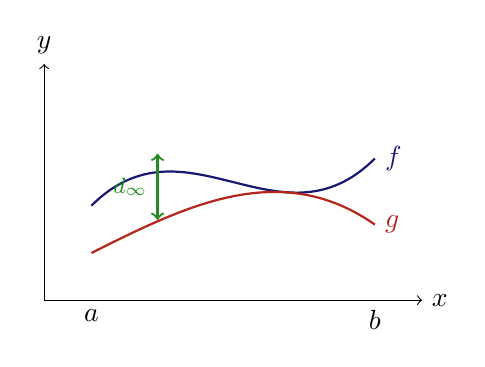
\begin{tikzpicture}[scale=1.2]
% \begin{ai-tikz-planner-invisible-content}
% 1. Background: Axes.
% 2. Midground: Two continuous functions f and g.
% 3. Foreground: A vertical bar showing the maximum difference for d_infinity.
% \end{ai-tikz-planner-invisible-content}
    % Axes
    \draw[->] (0,0) -- (4,0) node[right] {$x$};
    \draw[->] (0,0) -- (0,2.5) node[above] {$y$};
    \node[below] at (0.5, 0) {$a$};
    \node[below] at (3.5, 0) {$b$};

    % Functions
    \draw[thick, MidnightBlue] (0.5, 1) .. controls (1.5, 2) and (2.5, 0.5) .. (3.5, 1.5) node[right] {$f$};
    \draw[thick, BrickRed] (0.5, 0.5) .. controls (1.5, 1) and (2.5, 1.5) .. (3.5, 0.8) node[right] {$g$};
    
    % Max difference
    \draw[<->, thick, ForestGreen] (1.2, 1.55) -- (1.2, 0.85) node[midway, left] {\footnotesize $d_\infty$};
\end{tikzpicture}
\end{center}

\begin{explanation-of-steps}
The $L^\infty$ metric measures the \qt{worst-case} difference between two functions, while the $L^2$ metric provides an \qt{average} measure of their difference over the entire interval. Both satisfy the metric axioms, demonstrating that the concept of distance extends far beyond simple points in space.
\end{explanation-of-steps}
\end{math-stroke}
